\subsection{Task 1b: Three ways to count}

\textbf{Implementation} (\texttt{Task1b.java}). The whole file is first loaded into an
\texttt{int[]} of 50\,000\,000 elements (not measured). The array is divided into equal
contiguous parts, one per thread, and the program is run with
\texttt{--mode unsync|lock|local}. By default it uses as many threads as there are logical
processors, \texttt{Runtime.availableProcessors()}~=~12 on my laptop. The three versions differ
only in where a thread adds one to a counter:

\begin{lstlisting}
// 1: shared counters (plain fields of one shared object), no synchronisation
if (v < 0) shared.negative++; else if (v > 0) shared.positive++; else shared.zero++;

// 2: the same shared counters, every increment under a ReentrantLock
lock.lock();
try { if (v < 0) shared.negative++; else if (v > 0) shared.positive++; else shared.zero++; }
finally { lock.unlock(); }

// 3: local variables of the thread; written to its own Counts once, summed after join()
if (v < 0) negative++; else if (v > 0) positive++; else zero++;
\end{lstlisting}

Table~\ref{tab:1b-runs} shows every run with 12 threads (version~1 three times, as required, and
the other versions three times as well). Figure~\ref{fig:1b} and Table~\ref{tab:1b-threads}
show the three versions for all thread counts.

\begin{table}[H]
\centering\footnotesize\setlength{\tabcolsep}{4pt}
\begin{tabular}{lrrrrrrc}
\toprule
Version & Run & Time (ms) & Negative & Positive & Zero & Total & Correct \\
\midrule
1: shared, no sync & 1 & 330.1 & 3,369,126 & 3,360,083 & 25 & 6,729,234 & \textbf{no} \\
1: shared, no sync & 2 & 348.5 & 3,954,164 & 3,943,448 & 25 & 7,897,637 & \textbf{no} \\
1: shared, no sync & 3 & 331.2 & 3,402,233 & 3,391,194 & 25 & 6,793,452 & \textbf{no} \\
2: shared + lock & 1 & 794.6 & 25,001,107 & 24,998,868 & 25 & 50,000,000 & yes \\
2: shared + lock & 2 & 767.5 & 25,001,107 & 24,998,868 & 25 & 50,000,000 & yes \\
2: shared + lock & 3 & 736.1 & 25,001,107 & 24,998,868 & 25 & 50,000,000 & yes \\
3: per-thread counters & 1 & 72.7 & 25,001,107 & 24,998,868 & 25 & 50,000,000 & yes \\
3: per-thread counters & 2 & 83.3 & 25,001,107 & 24,998,868 & 25 & 50,000,000 & yes \\
3: per-thread counters & 3 & 74.8 & 25,001,107 & 24,998,868 & 25 & 50,000,000 & yes \\
\bottomrule
\end{tabular}

\caption{Task 1b with 12 threads (= logical processors): time and totals of every run. The correct
totals are 25\,001\,107 / 24\,998\,868 / 25 / 50\,000\,000}
\label{tab:1b-runs}
\end{table}

\begin{figure}[H]
\centering
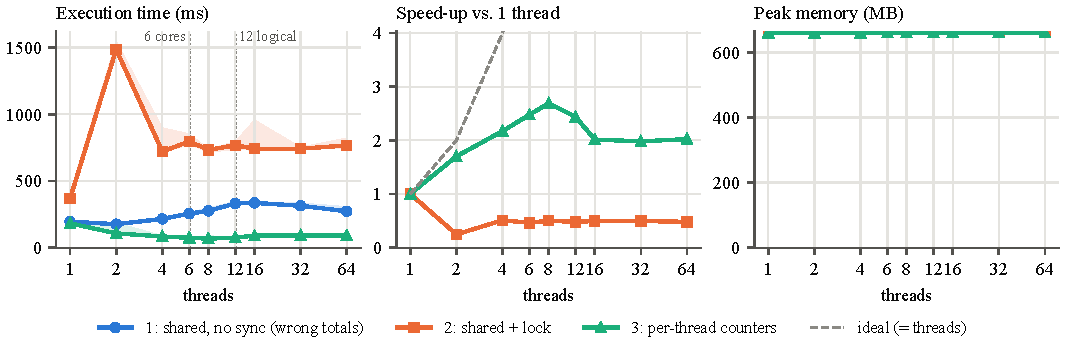
\includegraphics[width=\textwidth]{figures/task1b.pdf}
\caption{Task 1b: the three versions against the number of threads (median of 3 runs). Version 1
has no speed-up curve because its results are wrong. The peak-memory lines lie on top of each
other}
\label{fig:1b}
\end{figure}

\begin{table}[H]
\centering\small
\begin{tabular}{rrrrr}
\toprule
Threads & 1: no sync (ms) & 2: lock (ms) & 3: per-thread (ms) & 1: median total \\
\midrule
1 & 195 & 368 & 182 & 50.0M \\
2 & 176 & 1485 & 107 & 32.3M \\
4 & 215 & 721 & 84 & 21.3M \\
6 & 255 & 796 & 74 & 14.9M \\
8 & 276 & 733 & 68 & 12.2M \\
12 & 331 & 767 & 75 & 6.8M \\
16 & 336 & 741 & 90 & 7.2M \\
32 & 314 & 742 & 92 & 6.7M \\
64 & 273 & 765 & 90 & 6.6M \\
\bottomrule
\end{tabular}

\caption{Task 1b: median time of each version, and the median total counted by version 1 (it
should be 50.0M)}
\label{tab:1b-threads}
\end{table}

The peak memory is about 660\,MB for every version and thread count. It comes from loading the
array: the array grows by doubling while the file is read and is then trimmed to exactly
50\,000\,000 elements, so for a moment a 256\,MB and a 200\,MB array exist at the same time. The
counters themselves take a few bytes, so the memory does not depend on the version or the number
of threads.

\subsection{Task 1c: Producer and consumers}

\textbf{Implementation} (\texttt{Task1c.java}). The reader thread reads \texttt{numbers.txt}
line by line (\texttt{readLine()} of a \texttt{BufferedReader}) and collects the lines into \texttt{String[]} batches of
10\,000. It puts each batch into an \texttt{ArrayBlockingQueue} with capacity 100 batches, a
blocking queue from the Java library. \texttt{put()} blocks the reader while the queue is full,
and \texttt{take()} blocks a worker while the queue is empty. Java's \texttt{BlockingQueue} has no
\texttt{close()}, so the reader closes the queue another way. After the last batch it puts one
empty marker array (\texttt{END}) for every worker. The queue is FIFO, so a worker sees
\texttt{END} only after all real batches are taken, and then it stops. Every worker parses the
lines of its batches and counts into its own counters, which are added after \texttt{join()}. The
program also counts how often the reader found the queue full and how often a worker found it
empty, and the largest number of batches that were waiting in the queue.

\begin{figure}[H]
\centering
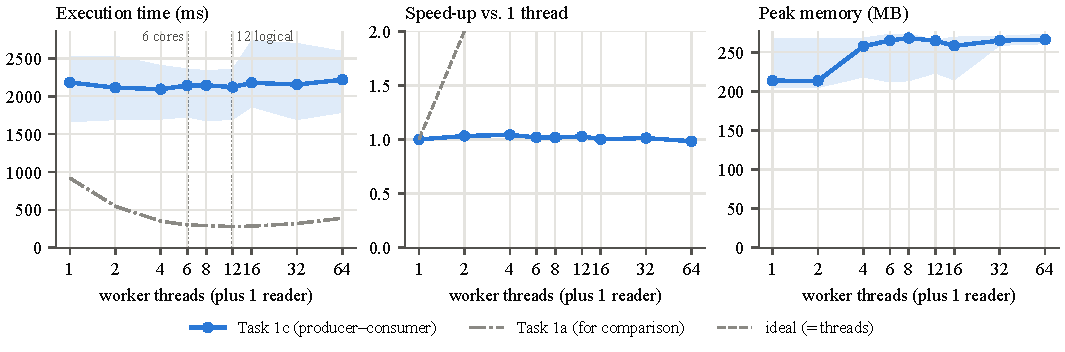
\includegraphics[width=\textwidth]{figures/task1c.pdf}
\caption{Task 1c: time, speed-up and peak memory against the number of workers (median of 5 runs;
the band shows the fastest and slowest run). The dash-dotted line is Task 1a}
\label{fig:1c}
\end{figure}

\begin{table}[H]
\centering\small
\begin{tabular}{rrrrr}
\toprule
Threads & Median time (ms) & Min--max (ms) & Speed-up & Peak memory (MB) \\
\midrule
1 & 2183 & 1664--2532 & 1.00 & 214 \\
2 & 2114 & 1691--2532 & 1.03 & 214 \\
4 & 2094 & 1699--2408 & 1.04 & 258 \\
6 & 2143 & 1727--2362 & 1.02 & 265 \\
8 & 2146 & 1678--2340 & 1.02 & 268 \\
12 & 2122 & 1694--2357 & 1.03 & 265 \\
16 & 2179 & 1863--2736 & 1.00 & 258 \\
32 & 2155 & 1693--2698 & 1.01 & 265 \\
64 & 2220 & 1788--2594 & 0.98 & 266 \\
\bottomrule
\end{tabular}

\caption{Task 1c results}
\label{tab:1c}
\end{table}

\begin{table}[H]
\centering\small
\begin{tabular}{rrrr}
\toprule
Workers & Worker waits (empty queue) & Reader waits (full queue) & Max batches in queue \\
\midrule
1 & 4975 & 0 & 48 \\
2 & 4999 & 0 & 6 \\
4 & 5001 & 0 & 6 \\
6 & 5003 & 0 & 4 \\
8 & 5006 & 0 & 5 \\
12 & 5011 & 0 & 1 \\
16 & 5012 & 0 & 2 \\
32 & 5029 & 0 & 2 \\
64 & 5061 & 0 & 5 \\
\bottomrule
\end{tabular}

\caption{Task 1c: how the queue was used (the file gives 5\,000 batches; waits are medians of 5 runs,
the queue length is the largest over the runs)}
\label{tab:1c-waits}
\end{table}

To answer question 6 by measurement and not only in words, I also ran Task 1c with batches of a
single line (\texttt{--batch 1}) and with a queue without a size limit (\texttt{--capacity 0}, which
uses a \texttt{LinkedBlockingQueue}), with 1, 4 and 12 workers (Table~\ref{tab:1c-var}, one run each;
the rows with batch 10\,000 and limit 100 are the medians from Table~\ref{tab:1c}).

\begin{table}[H]
\centering\footnotesize\setlength{\tabcolsep}{4pt}
\begin{tabular}{rrrrrrr}
\toprule
Batch (lines) & Queue limit & Workers & Time (ms) & Peak memory (MB) & Max batches in queue & Worker waits \\
\midrule
10,000 & 100 & 1 & 2183 & 214 & 48 & 4975 \\
1 & 100 & 1 & 13377 & 207 & 100 & 1428281 \\
10,000 & no limit & 1 & 2191 & 358 & 65 & 4475 \\
10,000 & 100 & 4 & 2094 & 258 & 6 & 5001 \\
1 & 100 & 4 & 19320 & 205 & 100 & 963760 \\
10,000 & no limit & 4 & 2143 & 258 & 1 & 5003 \\
10,000 & 100 & 12 & 2122 & 265 & 1 & 5011 \\
1 & 100 & 12 & 42159 & 205 & 100 & 932549 \\
10,000 & no limit & 12 & 2094 & 269 & 2 & 5011 \\
\bottomrule
\end{tabular}

\caption{Task 1c with other batch sizes and queue limits}
\label{tab:1c-var}
\end{table}

\subsection{Answers to the questions of Task 1}

\q{1. At which number of threads does the speed-up stop growing? Relate it to your physical cores
and logical processors.}
The speed-up grows fast up to 6 threads, my 6 physical cores (3.05$\times$), then only a little up
to 12, my 12 logical processors (3.30$\times$, the best). Two logical processors of one core share
its execution units, so the second one adds only 8\,\%. Above 12 the time grows again.

\q{2. Why do 32 and 64 threads not help? Are they slower, and why?}
They are slower: 319\,ms and 391\,ms against 279\,ms with 12 threads. Only 12 threads can run at
the same time, so the operating system has to switch between the others, and every switch, thread
start and extra read buffer only adds time.

\q{3. Does the peak memory depend on the number of threads? Why?}
A little in Task 1a: 42\,MB with 1 thread and 108\,MB with 64, about 1\,MB per thread, because every
thread has its own 1\,MiB read buffer and stack. In Task 1b (about 660\,MB, the loaded array) and
Task 1c (214--268\,MB, the queue and the strings) it does not depend on the threads.

\q{4. Rank the three versions of Task 1b by time. Which of them are correct? Explain each result.}
With 12 threads: per-thread counters about 75\,ms, no synchronisation about 330\,ms, lock about
770\,ms. Only the lock and the per-thread versions are correct.
\begin{itemize}
\item \emph{No synchronisation}: wrong, 6.7--7.9 million instead of 50 million. \texttt{counter++}
is read, add, write; two threads read the same value and one increment is lost.
\item \emph{Lock}: correct, but only one thread at a time can count, so it is slower than one
thread alone (368\,ms).
\item \emph{Per-thread counters}: correct and fastest, because the threads share nothing while
counting and the results are added once after \texttt{join()}.
\end{itemize}

\q{5. Compare Task 1c with Task 1a. Which one is faster, and why? At which number of workers
does Task 1c stop getting faster?}
Task 1a is faster: 279\,ms against about 2\,100\,ms. In Task 1c only one reader reads the file
and creates the strings, and the workers wait for it (they found the queue empty for almost every
batch). So Task 1c does not get faster after 1 worker.

\q{6. What would happen with batches of a single line? And with a queue that has no size limit?}
With batches of one line every line needs its own queue operation and lock, so it was 6--20 times
slower (13\,s with 1 worker, 42\,s with 12). A queue with no limit gave the same time here, because
the reader is the slow one; but if the workers were slower, the whole file could pile up in memory
(about 2.5\,GB). The limit of 100 batches makes the reader wait and keeps the memory small.
